\chapter{Statistics}\label{sec:statistics}

Every scientific investigation starts with a hypothesis that is to be tested empirically. The main objective is to evaluate if the proposed hypothesis agrees or disagrees with observed data, to either accept or reject it against the null-hypothesis which represents a baseline scenario where only known phenomena are presumed to occur.

A key metric that quantifies this is the p-value that arises within hypothesis testing. Test results of an experiment follow some probability density function. Assuming some hypothesis, the p-value is the integrated probability for test results compatible with this hypothesis and ergo measuring the compatibility of the observation to the assumption. In other words if the experiment where to be repeated it gives the probability that the result favors the proposed hypothesis.

In the field of high energy physics a framework has been developed specifically for this task. This section begins to lay out the mathematical fundamentals of the approach and explains its implementation in \textsc{pyhf} \citep{pyhf,pyhf_joss}. The following is based on \citep{cowan2011asymptotic,behnke2013data,pyhf}.

\section{Profile Likelihood Ratio}\label{sec:likelihood}
The statistical model needs to reflect the compatibility of predictions with the observed collision events. This can be quantified by a likelihood $L(\bm{x} | \bm{\phi})$ which is a probability for an observation $\bm{x}$ under a given set of parameters $\bm{\phi}$ that govern the predictions. Given that this is a counting experiment bins of a histogram $\bm{h}=(h_1,...,h_N)$ are the main tool of analysis.

The observation can be subdivided $\bm{x}=(\bm{n},\bm{a})$ into observable histograms $\bm{n}$ and auxiliary measurements. Observable histograms could be the invariant mass of a particle on the other hand auxiliary measurement histograms $\bm{a}$ can be any additional observable that assist in constraining the model. For instance they can be a measurement of a kinematic variable in a phase space region where only background is expected. It should be noted that these auxiliary measurements are not equivalent to the inclusion of uncertainties into the model. The treatment of uncertainties is addressed separately in section \ref{sec:histfactory_model}.

Another useful splitting for the set of parameters $\bm{\phi}=(\bm{\psi},\bm{\Theta})$ into so-called parameters of interest $\bm{\psi}$ and nuisance parameters $\bm{\Theta}$. For this section only one parameter of interest is considered, the signal strength $\mu$.

The bin contents can then be expressed in terms of the amount of signal $s_i(\bm{\Theta})$ and background $b_i(\bm{\Theta})$ in bin $i$ that depend on the nuisance parameters. The prediction (expectation value) of the histogram bins of the observable $n_i$ can then be expressed as
\begin{equation} \label{eq:n_i}
    \langle n_i(\mu,\bm{\Theta})\rangle = \mu s_i(\bm{\Theta}) +b_i(\bm{\Theta}).
\end{equation}
Similarly for auxiliary measurement bins $a_i$ their expectation value are calculable from some function $u_i(\bm{\Theta})$ modeling some observable and is also dependent on the nuisance parameters
\begin{equation} \label{eq:a_i}
    \langle a_i(\bm{\Theta}) \rangle = u_i(\bm{\Theta}).
\end{equation}
Since this is a counting experiment in which events occur at a constant mean rate and independently of time each bin follows a Poisson distribution
\begin{equation}\label{eq:poisson}
    P(r,k)=\frac{r^k e^{-r}}{k!}.
\end{equation}
$r$ is the expected rate of occurrences which translates as the prediction whereas $k$ are the actual measured occurrences. A likelihood can then be constructed from a product of Poisson probabilities
\begin{equation}\label{eq:likelihood}
    L(\mu,\bm{\Theta})=
    \prod_{j=1}^N \frac{(\mu s_j(\bm{\Theta}) + b_j(\bm{\Theta}))^{n_j}}{n_j !} e^{-(\mu s_j(\bm{\Theta}) + b_j(\bm{\Theta}))}
    \prod_{k=1}^M \frac{u_k(\bm{\Theta})^{a_k}}{a_k!} e^{-u_k(\bm{\Theta})}.
\end{equation}
The last product can also be thought of penalizing the likelihood if e.g. an auxiliary measurement displays a very improbable value for some quantity. To test for a hypothesized value of $\mu$, the best choice according to the Neyman-Pearson lemma \citep{behnke2013data}, is the profile likelihood ratio that reduces the dependence to the parameter(s) of interest
\begin{equation}\label{eq:likelihood_ratio}
    \lambda(\mu)=
    \frac{L(\mu,\hat{\hat{\bm{\Theta}}})}
    {L(\hat{\mu},\hat{\bm{\Theta}})}.
\end{equation}
The denominator is the unconditional maximum likelihood estimate so that $\hat{\mu}$ and $\hat{\bm{\Theta}}$ both are free to vary to maximize $L$, whereas the numerator is the found maximum likelihood conditioned on some chosen $\mu$ and the set of nuisance parameters $\hat{\hat{\bm{\Theta}}}$ that maximize the likelihood for that particular $\mu$. This definition gives $0 \leq \lambda \leq 1$ where $\lambda = 1$ corresponds to perfect agreement of the hypothesized value of $\mu$ to the model.

\section{Test Statistic and p-value}
To test for alternative hypotheses it is useful to transform the profile likelihood into a test statistic
\begin{equation}
    t(\mu)=-2\ln \lambda(\mu).
\end{equation}
This translates to $t \rightarrow 0$ as increasing agreement and $t \rightarrow \infty$ as decreasing agreement to the model. A right-tail p-value can then be calculated from the probability density function of the test statistic: \ac{pdf}$(t) = f(t | \mu)$
\begin{equation}\label{eq:p-value}
    p= \int_{t_\text{obs}}^{\infty}
    f(t | \mu) \mathrm{d}t
\end{equation}
$t_\text{obs}$ is the test statistic $t$ evaluated at the observed data which means replacing the predictions in the likelihood of the numerator of equation \ref{eq:likelihood_ratio} with the values observed in data. Similar to the \ac{pdf} of a standard normal distribution the \ac{pdf} in this context quantifies how probable a particular value of the test statistic $t$ is under a fixed value of the signal strength. This essentially measures how frequently a particular value of $t$ occurs in comparison to all other possible values that $t$ can take.

To calculate p-values the integral of equation \ref{eq:p-value} must be solved. The test statistic's specific form is useful because of existing approximations for $f(t | \mu)$ \citep{cowan2011asymptotic}. Let $f(t | \mu')$ be the probability distribution for the true strength parameter $\mu'$. \citet{wald1943tests} demonstrated that for a single parameter of interest the test statistic is equivalent to a normalized sum of squared distances between the tested parameter $\mu$ and its maximum likelihood estimate $\hat{\mu}$
\begin{equation}
    t(\mu)=-2\ln \lambda(\mu)=
    \left(\frac{\mu-\hat{\mu}}{\sigma_{\hat{\mu}}} \right)^2
    + \mathcal{O}(\frac{1}{\sqrt{N}}).
\end{equation}
The maximum likelihood estimate $\hat{\mu}$ is in the large sample limit normally distributed around their true value $\mu'$ with standard deviation $\sigma_{\hat{\mu}}$. This is the definition of a $\chi$-squared distribution with one degree of freedom. It can be shown that \citep{cowan2011asymptotic} the \ac{pdf} of $t$ is  asymptotically follows
\begin{equation}\label{eq:chi-square}
    f(t | \mu)=\frac{1}{2\sqrt{t}}\frac{1}{\sqrt{2\pi}}
    \left[
        \exp\left(-\frac{1}{2}\left(\sqrt{t}+\sqrt{\Lambda}_\mu\right)\right)
        +
        \exp\left(-\frac{1}{2}\left(\sqrt{t}-\sqrt{\Lambda}_\mu\right)\right)
        \right],
\end{equation}
with the non-centrality parameter as the normalized distance between the tested $\mu$ and true parameter of interest $\mu'$
\begin{equation}
    \Lambda_\mu=\frac{(\mu-\mu')^2}{\sigma^2}.
\end{equation}
Figure \ref{fig:test_stat_example} illustrates these steps. Being able to calculate p-values allows to state how likely it is that the proposed hypothesis is reflected by the observed data. In other words, the p-value represents the probability, how incompatible the proposed hypothesis or prediction is with the observation.
\begin{figure}
    \centering
    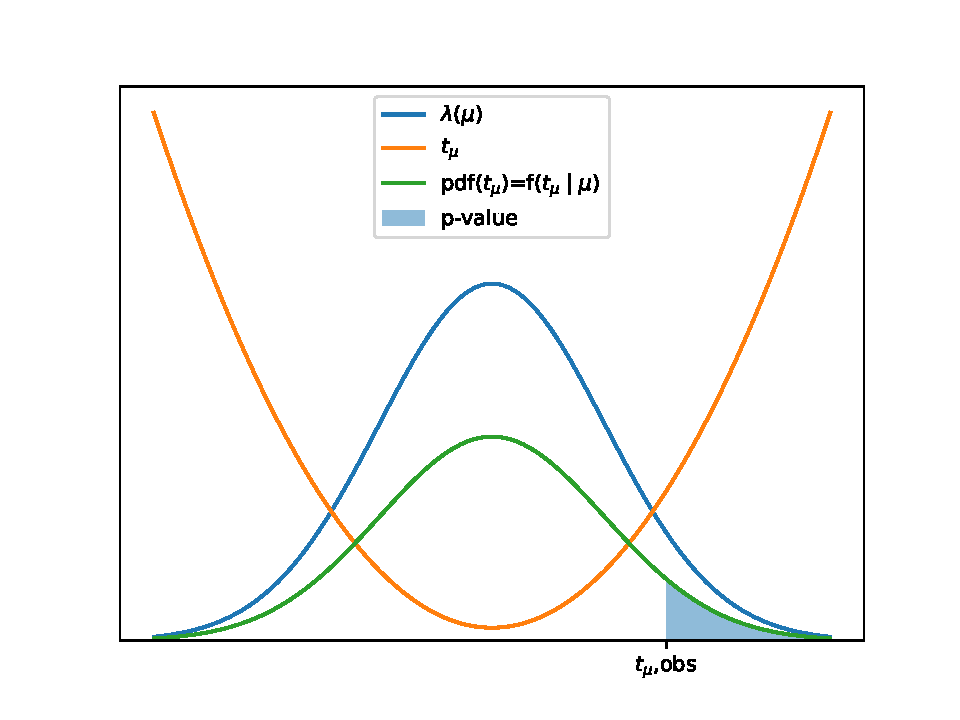
\includegraphics[width=0.8\textwidth]{test_stat_example.pdf}
    \caption[]{A sketch to follow the steps to calculate p-values. (\textbf{left}) The profile likelihood ({\color[HTML]{1f77b4}{$\bm{\diagup}$}}) has essentially some hill-like form with a maximum at ${\lambda(\hat{\mu},\hat{\bm{\Theta}})}$. The test statistic $t$ ({\color[HTML]{ff7f0e}{$\bm{\diagup}$}}) is calculated as $-2\mathrm{ln}(\lambda)$. (\textbf{right}) For one parameter of interest in the large sample limit $f(t | \mu)$ from equation \ref{eq:chi-square} follows a non-central chi-squared distribution with one degree of freedom. The blue shaded area under the \acp{pdf} is a right hand sided p-value.}
    \label{fig:test_stat_example}
\end{figure}

In the scientific community a p-value of 0.05 is commonly accepted as significant. Though particle physicists only claim discovery of a new phenomenon for $p$ < \qty{2.87e-7}{} corresponding to 5 standard deviations of the standard normal distribution and exclude hypotheses if the p-value is not below 2 standard deviations of the standard normal distribution $p$ $\lesssim$ \qty{0.05}{}. A key consideration is that $t$ can assume negative values for $\mu$ which might be non-physical depending on the context. This is handled by cutting off the test statistic for undesired behavior. An example of an adjusted test statistic for setting upper limits is
\begin{equation}
    q_\mu=
    \begin{cases}
        -2\ln \lambda(\mu) & \hat{\mu}\leq\mu \\
        0                  & \hat{\mu}> \mu
    \end{cases}.
\end{equation}
Here if a tested signal strength $\mu$ is not larger than the maximum estimate it would not be regarded as less compatible and is therefore set to zero. Various cases and approximations of \acp{pdf} in different scenarios are detailed in \citep{cowan2011asymptotic}.

\section{The CL$_s$ value}\label{sec:cls}
Particle physicists typically concentrate on two key aspects when performing statistical tests to discover new phenomena: the accurate modeling of known backgrounds and whether there is evidence in the observations for a new phenomenon. This involves assessing two distinct hypotheses: a background only ($b$) and one that involves signal and background ($s+b$). Each will result in a p-value of their own.

For example, a p-value of $p_{b} = 0$ would indicate a perfect modeling of the background model reflected in observational data, meaning that known phenomena have been accurately accounted for. Conversely, a p-value of $p_{s+b} < 0.05$ might signal the presence of new phenomena, such as previously undiscovered physics.

To synthesize these two aspects into a unified metric particle physicists developed a pseudo Confidence Level/p-value referred to as CL$_s$. This measure not only considers the potential presence of new phenomena but also the accuracy of the background modeling.
\begin{equation}
    \mathrm{CL}_s=\frac{p_{s+b}}{1-p_{b}}=
    \frac
    {\int_{t_\text{obs}}^{\infty}
        f(t_{s+b} | \mu) \mathrm{d}t}
    {1-\int_{t_\text{obs}}^{\infty}
        f(t_{b} | \mu) \mathrm{d}t}.
\end{equation}
The numerator represents the p-value for the alternative hypothesis while the denominator p-value penalizes the CL$_s$ based on how compatible the background model is with the observational data.  This concept can also be understood visually from the first figure of the paper that introduced the CL$_s$ quantity \citep{read2002presentation} and is explained here in figure \ref{fig:cls}.
\begin{figure}
    \centering
    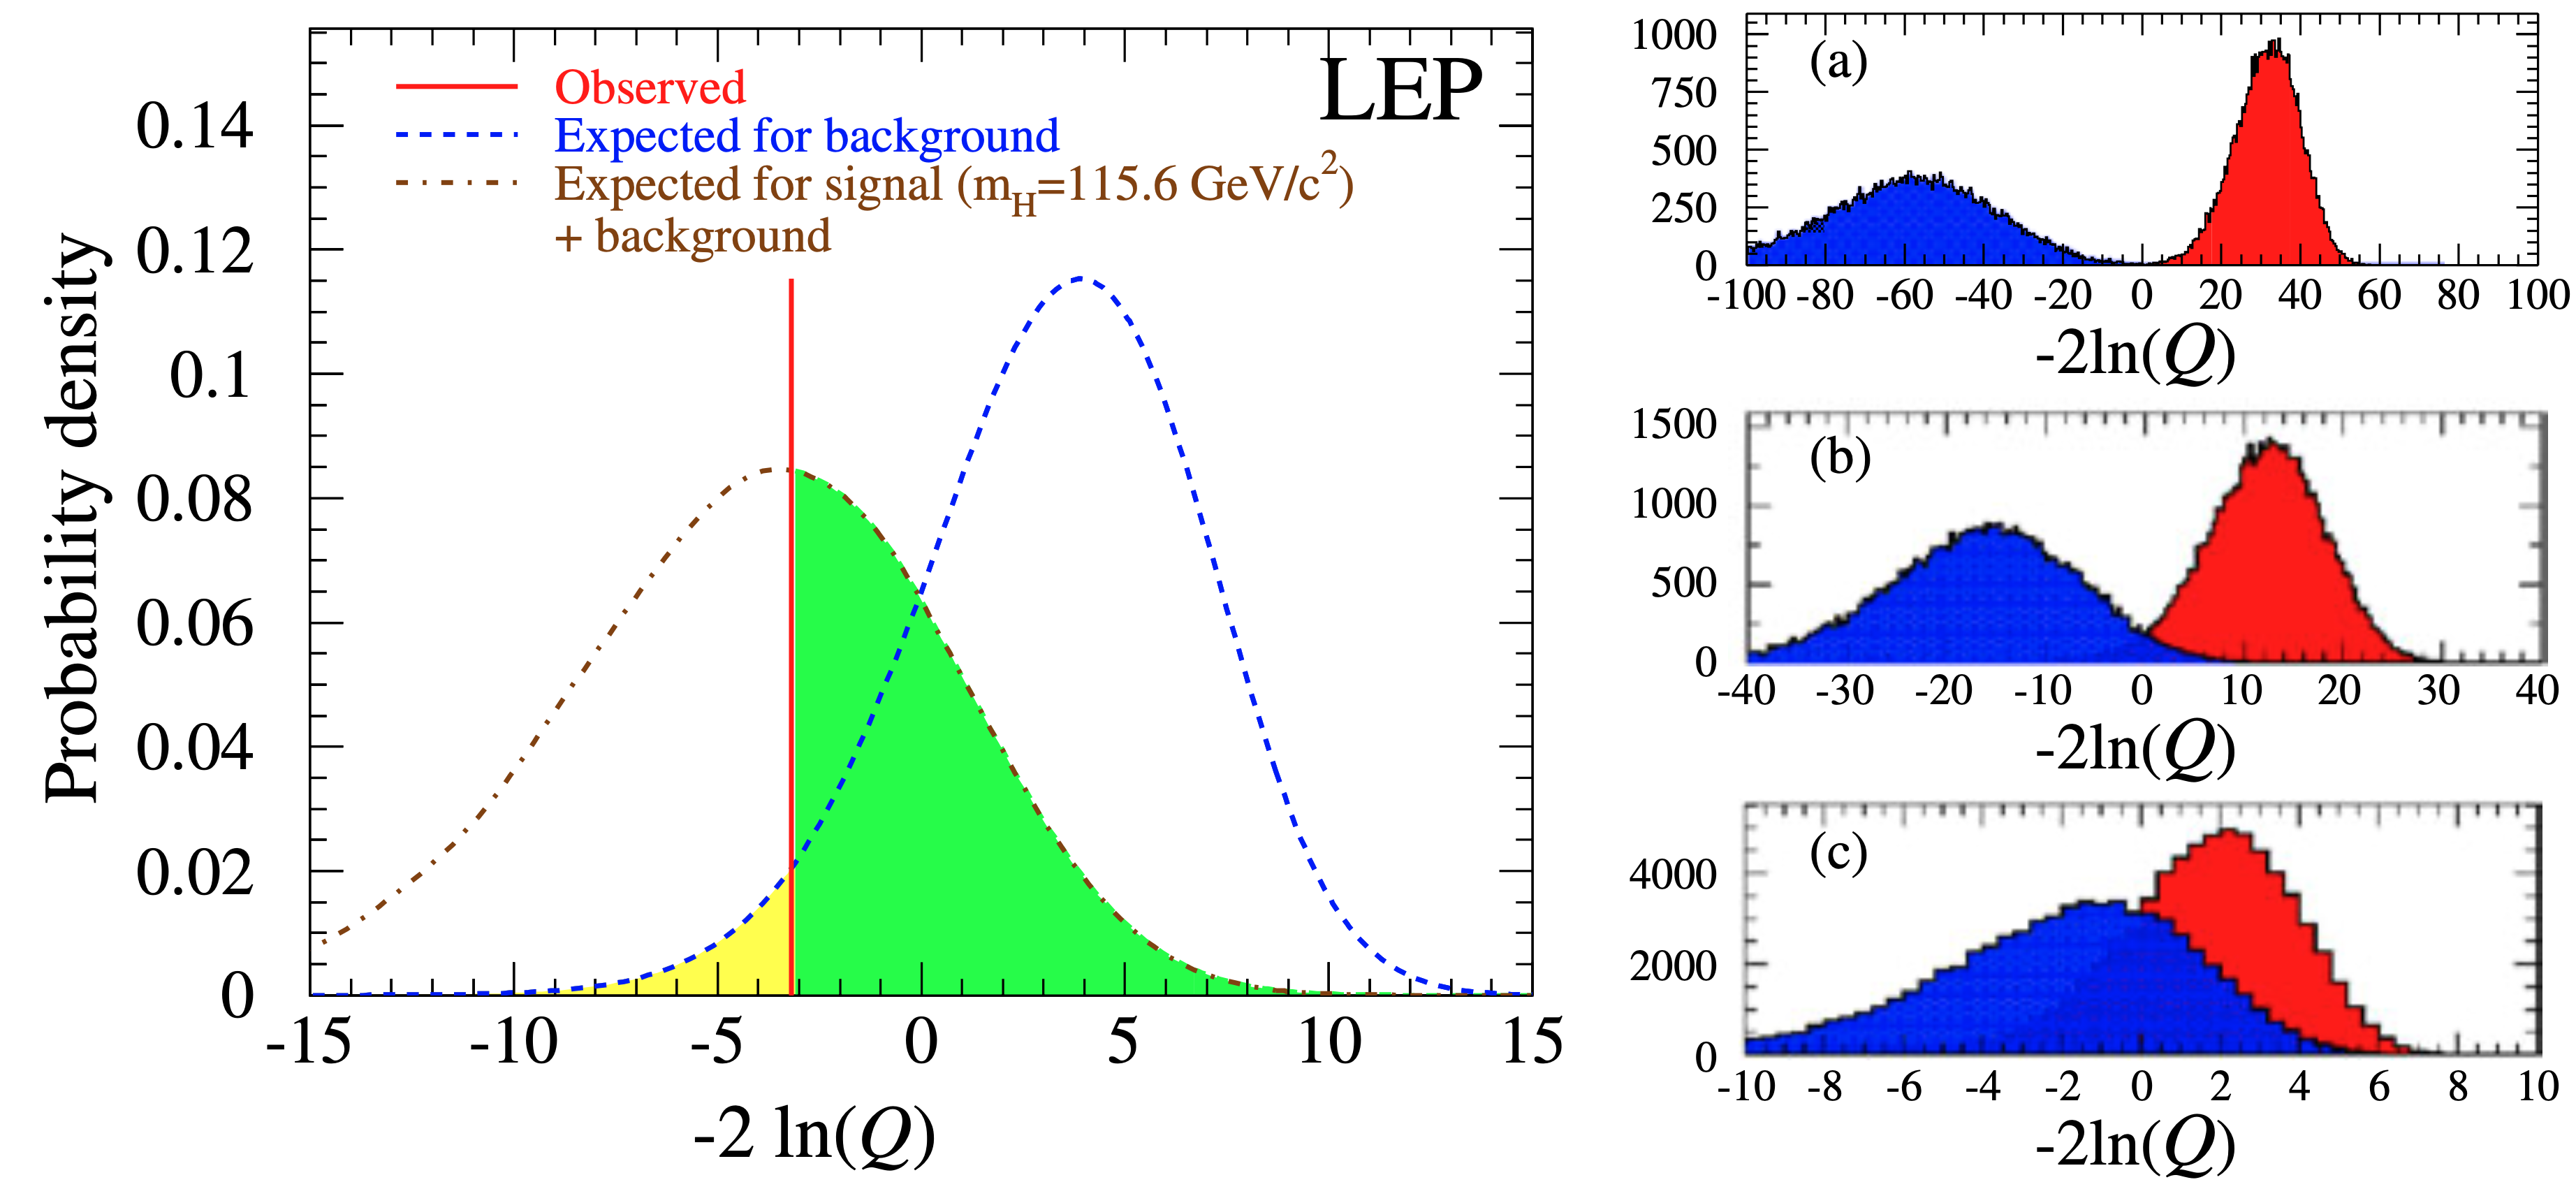
\includegraphics[width=1\textwidth]{cls.png}
    \caption[]{Probability density functions of test statistics from a Higgs search at LEP illustrating the calculation of p-values ($\lambda$ becomes $Q$). (\textbf{left}) The \acp{pdf}'s of the test statistic $f(t | \mu)$ of the signal + background ({\color[HTML]{804000}{$\bm{\diagup}$}}) and background ({\color[HTML]{2100FF}{$\bm{\diagup}$}}) only hypotheses. The p-value is calculated by integration from $t_\text{obs}$ (the red observed line ({\color[HTML]{FF0000}{$\bm{\diagup}$}})) to infinity (see eq. \ref{eq:p-value}). The green shaded area (\hexbox{00FF00}) corresponds to $p_{s+b}$ whereas the yellow area (\hexbox{FDFF02}) corresponds to $1-p_b$ since the integral over one whole \acp{pdf} is 1. (\textbf{right}) Degradation of search sensitivity from (a) to (c). Note that the colors of the \acp{pdf}'s change here to signal + background (\hexbox{2100FF}) and background only (\hexbox{FF0000}). For example putting the observation ($t_\text{obs}$) on the x-axis at 0 in these plots, one would get for plot (a) $p_{b}\approx 1$ and $p_{s+b}\approx 0$ resulting in a CL$_s\approx 0$, whereas with increasing overlap the CL$_s$ value increases and the sensitivity decreases. Adopted from \citep{read2002presentation}.}
    \label{fig:cls}
\end{figure}


\section{HistFactory}\label{sec:histfactory_model}
A widely-used model for constructing likelihoods as discussed in section \ref{sec:likelihood} is known as HistFactory \citep{cranmer2012histfactory}. This model is implemented in the \textsc{pyhf} toolkit \citep{pyhf} and the following section is primarily based on the introduction to HistFactory found in the \textsc{pyhf} documentation. HistFactory simplifies the process of building a likelihood by breaking it down into several fundamental components. To understand this it is helpful to consider a different categorization of the model parameters $\bm{\phi}$
\newcommand{\freeset}{\bm{\eta}}
\newcommand{\constrset}{\bm{\chi}}
\newcommand{\singleconstr}{\chi}
\newcommand{\channelcounts}{\bm{n}}
\newcommand{\auxdata}{\bm{a}}
\newcommand{\poiset}{\bm{\psi}}
\newcommand{\nuisset}{\bm{\theta}}
\newcommand{\fullset}{\bm{\phi}}
\newcommand{\singlefull}{\phi}
\begin{equation}
    L(\bm{x}|\fullset) \quad=\quad
    L(\bm{x}|\overbrace{\poiset}^{\llap{\text{parameters of interest}}},\underbrace{\nuisset}_{\llap{\text{nuisance parameters}}}) \quad=\quad
    L(\bm{x}|\overbrace{\freeset}^{\rlap{\text{free}}},\underbrace{\constrset}_{\rlap{\text{constrained}}}),
\end{equation}
Free parameters $\freeset$ are free to choose in the model and can be for example a cross-section of a process. Constrained parameters $\constrset$ are used to incorporate uncertainties into the likelihood to constrain it. Further there might be several histograms of an observable, for example measured in orthogonal kinematic regions, that are called channels $c$. Bins have the index $b$ here and constraint terms are denoted $c_{\singleconstr}$. The likelihood can thus be described by
\begin{equation}
    L(\channelcounts, \auxdata \,|\,\freeset,\constrset)
    = \underbrace{\color{blue}{\prod_{c\in\mathrm{\,channels}} \prod_{b \in \mathrm{\,bins}_c}
            \textrm{Pois} ( 
                \;\overbrace{n_{cb}}^{\llap{\text{\strut observed}\quad\;}}
            \,|\, \overbrace{\nu_{cb}\left(\freeset,\constrset\right)}^{\llap{\quad\text{\strut predicted}}}
            \;)}}_{\substack{\text{Simultaneous measurement}\\%
            \text{of multiple channels}}}
    \underbrace{\color{red}{\prod_{\singleconstr \in \constrset} c_{\singleconstr}(a_{\singleconstr} |\, \singleconstr)}}_{\substack{\text{constraint terms}\\%
            \text{for }\text{auxiliary measurements}}}.
            \label{eq:histfactory_likelihood}
\end{equation}
$\bm{n}$ and $\bm{a}$ are the observations auxiliary measurement hisograms as defined in section \ref{sec:likelihood}. The $n_{cb}$ is the observed bin content and $\nu_{cb}(\freeset,\constrset)$ the predicted bin content. $c_{\singleconstr}(a_{\singleconstr} |\, \singleconstr)$ are functions that calculate a probabilistic impact to the likelihood $L$ of uncertainties $a_\chi$ to constrain the parameter $\singleconstr$ and are discussed in detail section \ref{sec:constraint_terms}.

The prediction is a sum of nominal bin counts\footnote{also called rates, like in the definition of a Poisson distribution} $\nu_{scb}^0$ over all samples $s$ (e.g. $t\overline{t}$, multijet-background, etc.). These nominal bin counts are subject to uncertainties. Therefore the bin content can be varied within the bounds of these uncertainties. However the effect of this modification to the likelihood must be taken into account which is through the constraint terms. These penalize the likelihood proportional to the modification. Modifiers are discussed in detail in section \ref{sec:modifiers}. They enter the likelihood through linear modeling of the nominal bin content $\nu_{scb}^0$ with multiplicative $\kappa_{scb}$ and additive modifiers $\Delta_{scb}$ 
\begin{align}
    \nu_{cb}\left(\freeset,\constrset\right) & = \sum_{s\in\mathrm{\,samples}} \nu_{scb}\left(\freeset,\constrset\right)                                                                                                \\
                                             & = \sum_{s\in\mathrm{\,samples}}\underbrace{\left(\prod_{\kappa\in\,\bm{\kappa}} \kappa_{scb}\left(\freeset,\constrset\right)\right)}_{\text{multiplicative modifiers}}\,
    \Bigg(\nu_{scb}^0 + \underbrace{\sum_{\Delta\in\bm{\Delta}} \Delta_{scb}\left(\freeset,\constrset\right)}_{\text{additive modifiers}}\Bigg).
    \label{eq:modifier_equation}
\end{align}
The usefulness of this approach becomes clear when considering one uncertainty $a_\chi$ on a nominal bin count estimate $\nu_{scb}^0$. The main goal remains to maximize the overall likelihood $L$. This can be achieved via maximizing the Poisson probability (blue part in equation \ref{eq:histfactory_likelihood}) and at the same time keeping the constraint term (red part in equation \ref{eq:histfactory_likelihood}) large. It is illustrative to consider one nuisance parameter $\chi$ as a multiplicative modifier $\kappa_{scb}=\chi$ on $\nu_{scb}^0$. An optimum can be found by modifying the prediction to move closer to the observed value (blue part in equation \ref{eq:histfactory_likelihood}) while at the same time keeping the constraint term $c_\kappa(\kappa)$ (red part in equation \ref{eq:histfactory_likelihood}) controlled by the same $\chi$ at values where the penalization of the likelihood stays insignificant. This works well for example when $\kappa$ has a very large uncertainty rendering the constraint term's influence on the likelihood relatively small. 

\subsection{The Modifiers}\label{sec:modifiers}
In HistFactory there are by convention four types $\{\lambda,\mu,\gamma,\alpha\}$ of such multiplicative rate modifiers that are explained in this section. There are \textbf{free rate modifiers} for the luminosity $\lambda$ and signal strength $\mu$ that affect all bins equally
\begin{equation}
    \nu_{scb}(\mu)=\mu \nu_{scb}^0.
\end{equation}
These are bin-independent normalization factors and preserve the shape of the histogram.
Further there are \textbf{bin-wise modifiers} $\gamma_b$ (uncorrelated shape)
\begin{equation}
    \nu_{scb}(\gamma_b)=\gamma_b \nu_{scb}^0.
\end{equation}
These are useful for example to include uncertainties of a per bin data-driven background estimate. This type without a constraint term is not of much use as if there is only one sample or channel, the fit would always match the data perfectly.
In addition there exist \textbf{interpolation parameters $\alpha$} (shape factors) that enter the modeling through an interpolation function $\eta$ instead of being the factor itself. They exist in multiplicative versions
\begin{equation}
    \nu_{scb}(\alpha)=\eta(\alpha) \nu_{scb}^0,
\end{equation}
and additive versions
\begin{equation}
    \nu_{scb}(\alpha)=\nu_{scb}^0 + \eta(\alpha).
\end{equation}
This is useful to include systematic uncertainties. Typically they are known for one standard deviation of a bin count $\eta_{-1}=\nu_{scb}^\mathrm{1down}$ and $\eta_{1}=\nu_{scb}^\mathrm{1up}$ to the nominal value $\nu_{scb}^0$. These are then used to construct interpolation functions that modify the nominal value controlled by the nuisance parameter that also controls the constraint term $c_\alpha$ which is further explained in section \ref{sec:constraint_terms}. Thus one parameter controls the modification and constraint at a time.

In HistFactory there exists four of such interpolation functions. For those exist an identity operator
\begin{equation}
    \eta_0=\eta (\alpha=0) =
    \begin{cases}
        1 , & \text{multiplicative modifier, } (\kappa) \\
        0 , & \text{additive modifier, } (\lambda).
    \end{cases}
\end{equation}
One example of these interpolation functions that scales the bin count linearly over the known deviations $\eta_{-1}=\nu_{scb}^\mathrm{1down}$ and $\eta_{1}=\nu_{scb}^\mathrm{1up}$ is
\begin{equation}
    \eta_\mathrm{linear}(\alpha)=
    \begin{cases}
        \alpha(\eta_0 - \eta_1) ,    & \alpha>0 \\
        \alpha(\eta_0 - \eta_{-1}) , & \alpha<0
    \end{cases}
\end{equation}
This is illustrated in fig. \ref{fig:interp_func}(a). For the other ones see e.g. \citep{heinrich2019searches}. It is noted that $\alpha$ is the nuisance parameter and not the function $\eta(\alpha)$ and there is an associated constraint term $c_\alpha$ to each $\alpha$.
\begin{figure}
    \centering
    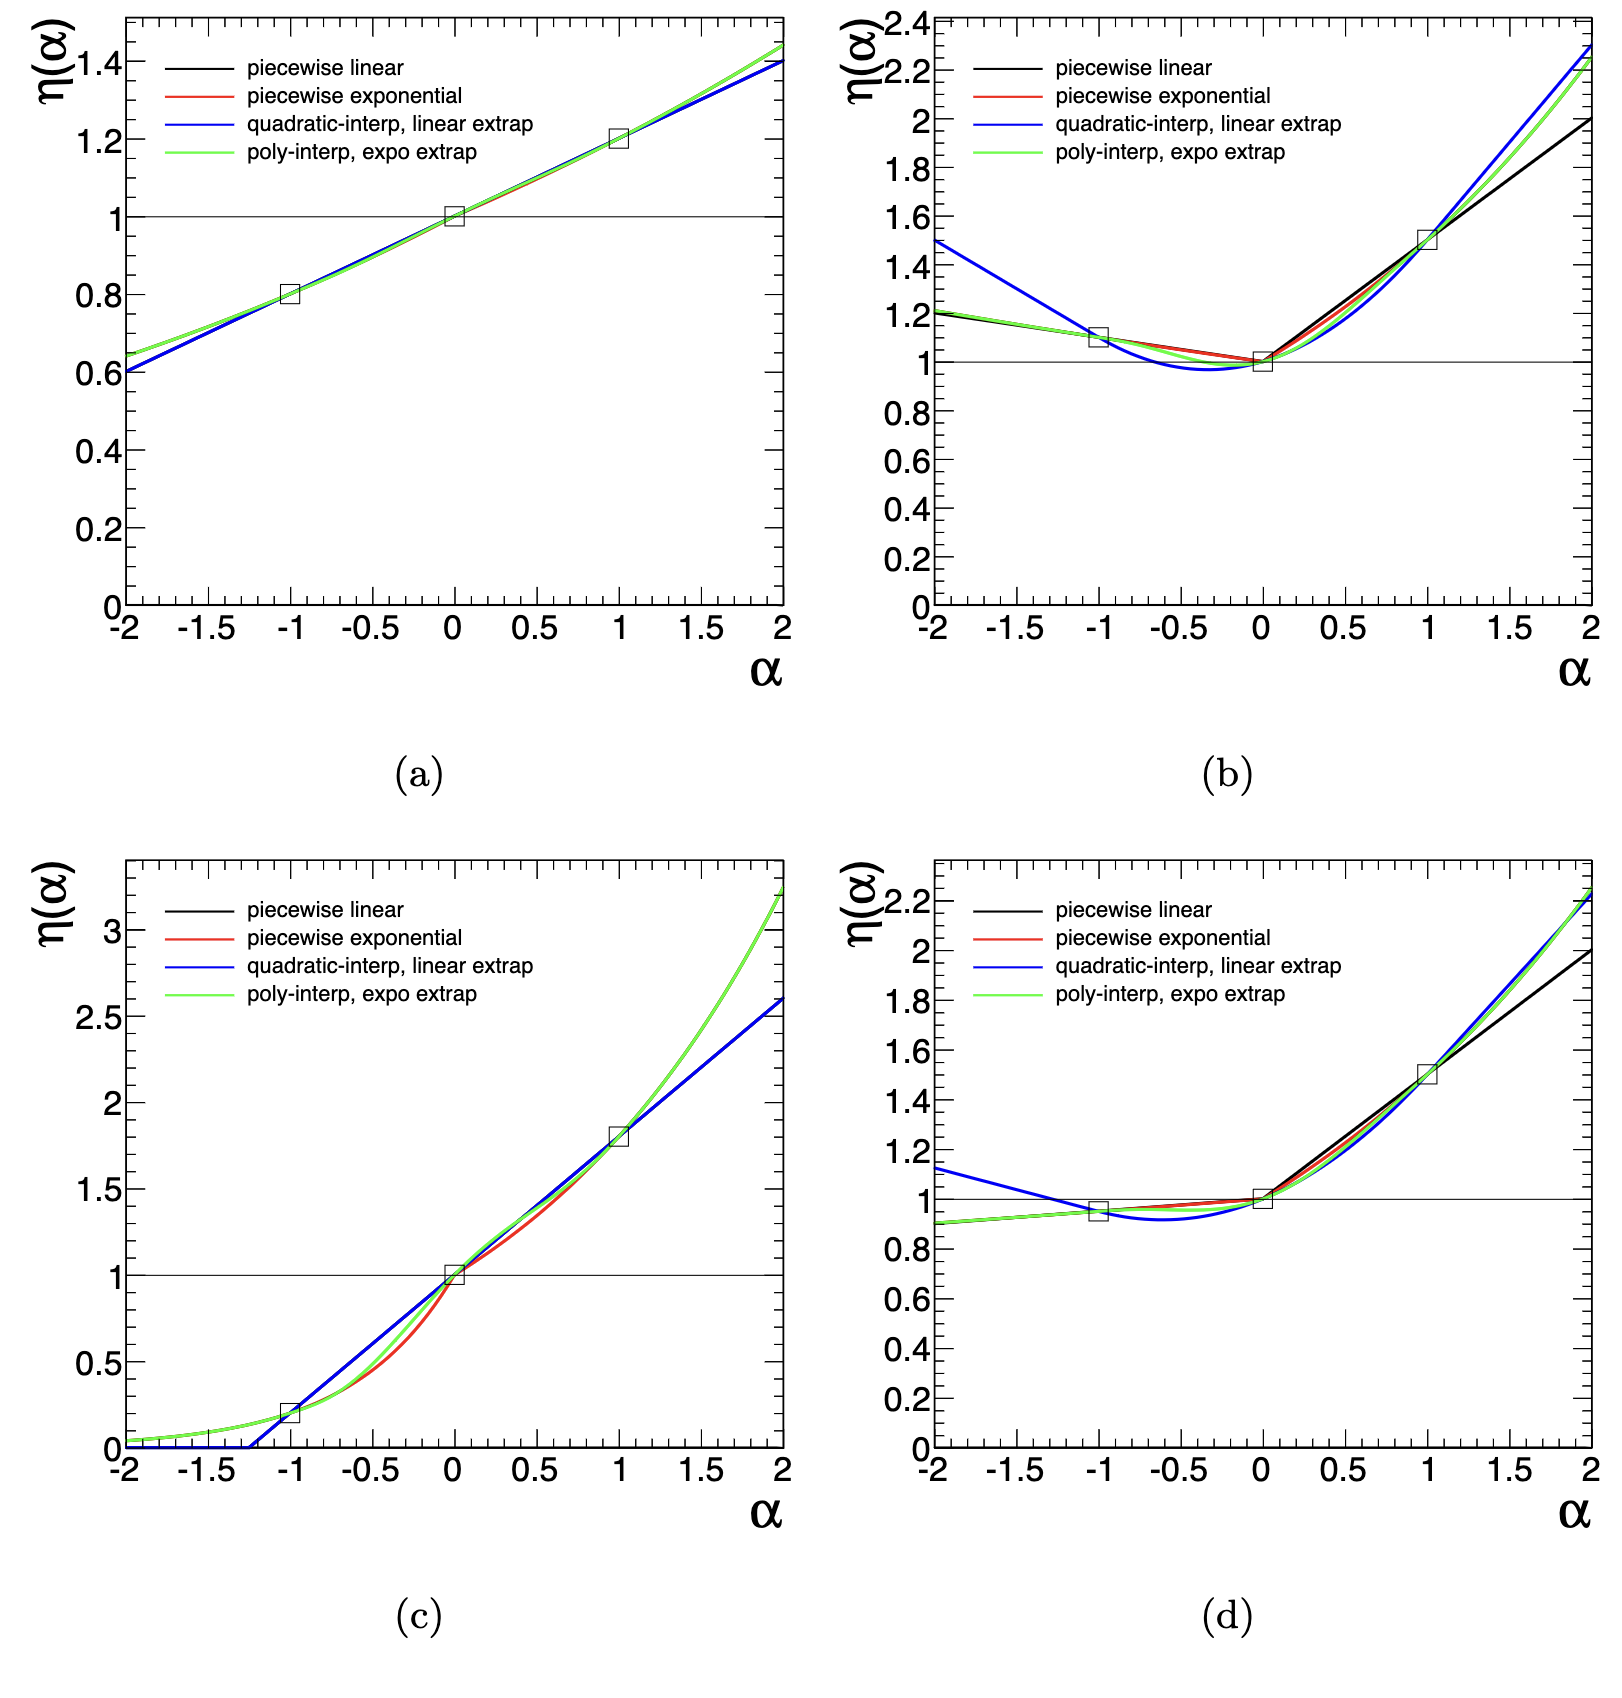
\includegraphics[width=.8\textwidth]{interp_func.png}
    \caption[]{The four interpolation functions $\eta(\alpha)$ for different up and down standard deviation values. For example in (a) the bin count will be scaled with a factor of 0.8 for an $\alpha=-1$ (1.2 for an $\alpha=1$). From \citep{cranmer2012histfactory}.}
    \label{fig:interp_func}
\end{figure}

\subsection{The constraint terms}\label{sec:constraint_terms}
Uncertainties are modeled either Gaussian or Poissonian. The Gaussian uncertainty implementation is straightforward as the standard deviation $\sigma$ appears in the definition of the Gaussian with mean $\mu$
\begin{equation}
    \text{Gaus}(\mu|x,\sigma)=\frac{1}{\sigma\sqrt{2\pi}}e^{-\frac{1}{2}\left(\frac{x-\mu}{\sigma}\right)^2}.
\end{equation}
So that the likelihood for a Gaussian uncertainty is constrained by a Gaussian scaled to one standard deviation controlled by the nuisance parameter $\alpha$: \mbox{$\mathrm{Gauss}(\alpha | a, \sigma=1)$}.

Similar to the Gaussian uncertainty for an uncertainty that is Poissonian distributed
\begin{equation}
    \text{Pois}(k|r)= \frac{r^k e^{-r}}{k!}.
\end{equation}
the nuisance parameter for a multiplicative factor $\kappa_{scb}=\gamma$ in equation \ref{eq:modifier_equation} should control the Poisson constraint term such that the uncertainty $\sigma$ is reflected by the variance of the Poisson $\text{Var}(\text{Pois})=r=\sigma^2$. This is achieved by scaling the distribution with a factor $f$ which is then solved for the one with the desired uncertainty by evaluating it at the nominal value of the multiplicative modifier $\gamma_0=1$ 
\begin{equation}
    \mathrm{Var}\left[\mathrm{Pois}(k=f\gamma_0 | r=f\gamma)\right]
    =
    r=f\gamma\;\stackrel{\gamma=\gamma_0}{=}\;f\gamma_0=(f\sigma)^2 
    \quad 
    \rightarrow \quad f=(1/\sigma^2).
\end{equation}
Thus a Poissonian constraint term for a multiplicative modifier $\gamma$ with uncertainty $\sigma$ reads \mbox{$\text{Pois}(k=\sigma^{-2}|r=\sigma^{-2}\gamma)$.} This completes the necessities for the HistFactory model. The different types of modifiers and their constraint terms are summarized in table \ref{tab:histfactory}.
\begin{table}[]
    \caption[]{Modifiers and constraint terms used in HistFactory implemented by \textsc{pyhf}. Note that the interpolation functions are called $f_p$ and $g_p$ here instead of $\eta$ as chosen in the full text. Input for the constraint terms are the corresponding uncertainties. Adapted from \citep{pyhf}.}
    \centering
    \resizebox{0.97\textwidth}{!}{
        \begin{tabular}{l|l|l|l}\label{tab:histfactory}
            Description          & Modification                                                                                            & Constraint Term $c_\singleconstr$                                                               & $c_\chi$ input                     \\
            \hline
            Uncorrelated Shape   & $\kappa_{scb}(\gamma_b) = \gamma_b$                                                                     & $\prod_b \mathrm{Pois}\left(k_b = \sigma_b^{-2}\middle|\,r_b = \sigma_b^{-2}\gamma_b\right)$ & $\sigma_{b}$                       \\
            Correlated Shape     & $\Delta_{scb}(\alpha) = f_p\left(\alpha\middle|\,\Delta_{scb,\alpha=-1},\Delta_{scb,\alpha = 1}\right)$ & $\displaystyle\mathrm{Gaus}\left(a = 0\middle|\,\alpha,\sigma = 1\right)$                       & $\Delta_{scb,\alpha=\pm1}$         \\
            Normalisation Unc.   & $\kappa_{scb}(\alpha) = g_p\left(\alpha\middle|\,\kappa_{scb,\alpha=-1},\kappa_{scb,\alpha=1}\right)$   & $\displaystyle\mathrm{Gaus}\left(a = 0\middle|\,\alpha,\sigma = 1\right)$                       & $\kappa_{scb,\alpha=\pm1}$         \\
            MC Stat. Uncertainty & $\kappa_{scb}(\gamma_b) = \gamma_b$                                                                     & $\prod_b \mathrm{Gaus}\left(a_{\gamma_b} = 1\middle|\,\gamma_b,\delta_b\right)$                 & $\delta_b^2 = \sum_s\delta^2_{sb}$ \\
            Luminosity           & $\kappa_{scb}(\lambda) = \lambda$                                                                       & $\displaystyle\mathrm{Gaus}\left(l = \lambda_0\middle|\,\lambda,\sigma_\lambda\right)$          & $\lambda_0,\sigma_\lambda$         \\
            Normalisation        & $\kappa_{scb}(\mu_b) = \mu_b$                                                                           &                                                                                                 &                                    \\
            Data-driven Shape    & $\kappa_{scb}(\gamma_b) = \gamma_b$                                                                     &                                                                                                 &                                    \\
        \end{tabular}
    }
\end{table}

